%!TEX root = ../trajectory-grouping.tex
Da das Ziel darin bestand, menschliche Intuition in ein mathematisches Modell zu überführen, haben \textcite{buchin2015} das Modell implementiert, auf unterschiedliche Testdaten angewandt und zur Visualisierung Videos\footnote{verfügbar unter \url{https://fstaals.net/grouping/}} produziert, an denen man gut überprüfen kann, ob dieses Ziel erreicht wurde.
Eine Menge von Trajektorien wurde dabei synthetisch basierend auf dem NetLogo-Modell  \cite{netlogo} erstellt, die zweite ist eine Teilmenge von Positionsdaten aus dem Starkey-Projekt \cite{starkey}, die die Bewegung von Hirschen, Elchen und Rindern im \emph{Starkey Experimental Forest} in Oregon erfassen. 
Diese Daten mussten zu diesem Zweck interpoliert werden, um die \cref{sec:trajek_reeb} eingeführten Bedingungen zu erfüllen.

\begin{figure}[hbtp]
    \Centering
    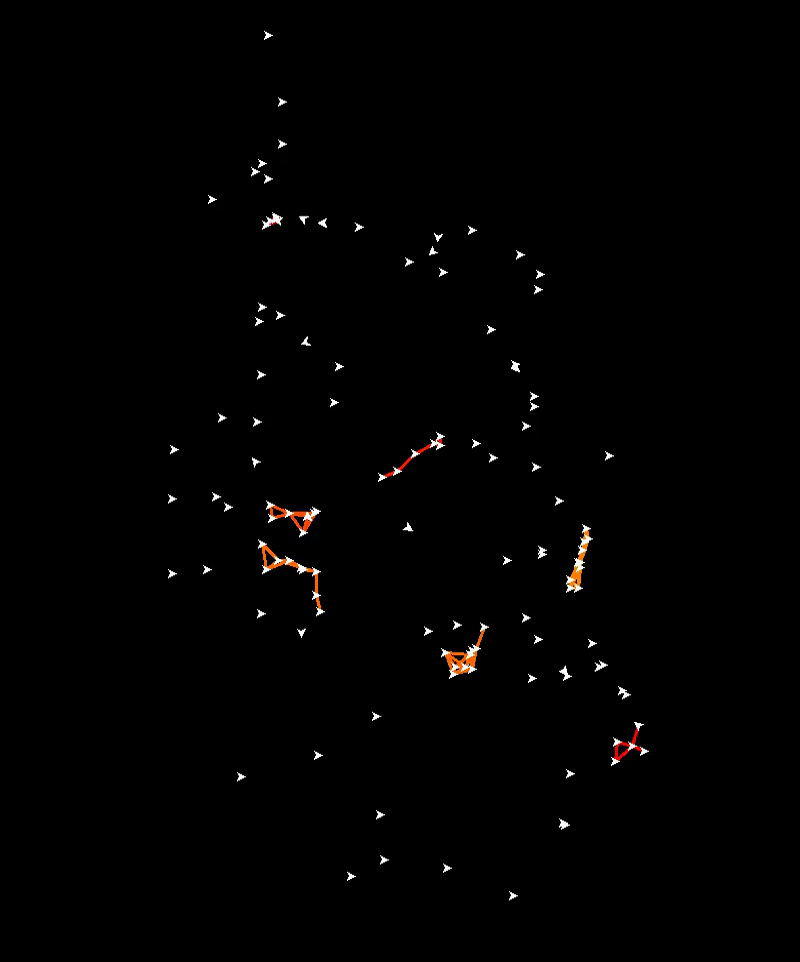
\includegraphics[width=.5\textwidth]{videos/starkey.png}
    \caption{Screenshot aus dem Video zu den Starkey-Daten.}\label{fig:starkey}
\end{figure}

Bei beiden Datensets zeigt sich, dass das Modell der menschlichen Intuition sehr gut entspricht.
\Cref{fig:starkey} zeigt einen Screenshot aus dem Video zu den Starkey-Daten, was dies schon verdeutlich -- erst in bewegten Bildern wird insbesondere die Einwirkung von $\delta$ aber wirklich klar.
Die Videos zeigen außerdem gut, wie die in \cref{cha:def_gruppe} besprochene Monotonie bei Variation der Parameter zum Tragen kommt.
